\documentclass[a4paper, 11pt]{article}
\usepackage[top=2cm, bottom=3cm, left = 2cm, right = 2cm]{geometry} 
\geometry{a4paper} 
\usepackage{textcomp}
\usepackage{graphicx} 
\usepackage{amsmath,amssymb}  
\usepackage{bm}  
\usepackage{memhfixc} 
\usepackage{fancyhdr}
\usepackage{enumerate}
\usepackage{tikz}
\usepackage{float}
\usepackage{booktabs}
\usepackage{xepersian}
\settextfont[Scale=1]{HM FNazli}
\setlatintextfont[Scale=.9]{Noto Sans}
\pagestyle{fancy}
\setlength{\headheight}{14pt}
\addtolength{\topmargin}{-2pt}

\title{
    گزارش نهایی محیط درستی‌سنجی برای
    \lr{Calc3}
}
\author{حسین افکار \\
۸۱۰۱۰۱۱۰۲}
%\date{}

\begin{document}
\maketitle
% \tableofcontents

\section{مقدمه}
در این پروژه یک محیط درستی‌سنجی برای ماشین‌حساب
\lr{Calc3}
نوشته‌ شده‌است


\tikzset{every picture/.style={line width=0.75pt}} %set default line width to 0.75pt        

\begin{figure}[H]
    \centering
    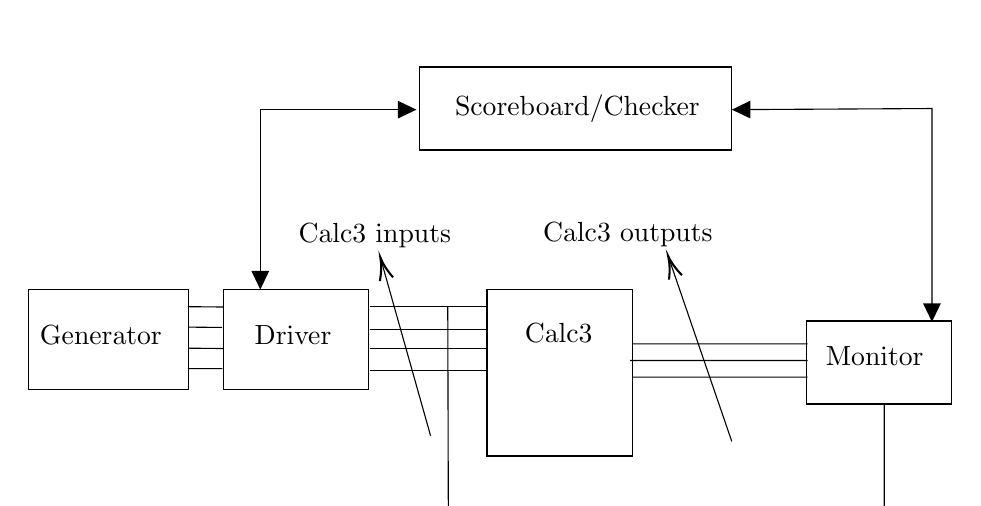
\begin{tikzpicture}[x=0.75pt,y=0.75pt,yscale=-1,xscale=1]
        %uncomment if require: \path (0,300); %set diagram left start at 0, and has height of 300
        
        %Shape: Rectangle [id:dp5697228224002759] 
        \draw   (289,122) -- (359,122) -- (359,202.03) -- (289,202.03) -- cycle ;
        %Straight Lines [id:da7189033070332109] 
        \draw    (232.47,130.03) -- (288.47,130.03) ;
        %Straight Lines [id:da3679326207032825] 
        \draw    (232.47,150.03) -- (288.47,150.03) ;
        %Straight Lines [id:da2467980653011279] 
        \draw    (232.47,161.03) -- (288.47,161.03) ;
        %Straight Lines [id:da40577994176378085] 
        \draw    (232.47,141.03) -- (288.47,141.03) ;
        %Shape: Rectangle [id:dp38730159512477735] 
        \draw   (162,122) -- (232,122) -- (232,170.03) -- (162,170.03) -- cycle ;
        %Straight Lines [id:da36353370229719206] 
        \draw    (261.83,192.24) -- (238.16,108.24) ;
        \draw [shift={(237.62,106.31)}, rotate = 74.26] [color={rgb, 255:red, 0; green, 0; blue, 0 }  ][line width=0.75]    (10.93,-3.29) .. controls (6.95,-1.4) and (3.31,-0.3) .. (0,0) .. controls (3.31,0.3) and (6.95,1.4) .. (10.93,3.29)   ;
        %Shape: Rectangle [id:dp16545893981577753] 
        \draw   (256.47,14.6) -- (406.7,14.6) -- (406.7,54.6) -- (256.47,54.6) -- cycle ;
        %Shape: Rectangle [id:dp07836664435212337] 
        \draw   (443,137) -- (513,137) -- (513,177) -- (443,177) -- cycle ;
        %Straight Lines [id:da34666593411430635] 
        \draw    (359,148) -- (443.47,148.03) ;
        %Straight Lines [id:da07946846692295706] 
        \draw    (359,164) -- (443.47,164.03) ;
        %Straight Lines [id:da8652457234478481] 
        \draw    (358,156) -- (443.47,156.03) ;
        %Straight Lines [id:da1385589744718032] 
        \draw    (270.12,130.24) -- (270.4,230.52) -- (480.4,230.81) -- (480.4,176.81) ;
        %Straight Lines [id:da4874312895005559] 
        \draw    (503.4,134.42) -- (503.4,34.62) -- (410,35.15) ;
        \draw [shift={(407,35.17)}, rotate = 359.68] [fill={rgb, 255:red, 0; green, 0; blue, 0 }  ][line width=0.08]  [draw opacity=0] (8.93,-4.29) -- (0,0) -- (8.93,4.29) -- cycle    ;
        \draw [shift={(503.4,137.42)}, rotate = 270] [fill={rgb, 255:red, 0; green, 0; blue, 0 }  ][line width=0.08]  [draw opacity=0] (8.93,-4.29) -- (0,0) -- (8.93,4.29) -- cycle    ;
        %Straight Lines [id:da6207609853062772] 
        \draw    (406.95,194.98) -- (376.93,107.54) ;
        \draw [shift={(376.28,105.64)}, rotate = 71.05] [color={rgb, 255:red, 0; green, 0; blue, 0 }  ][line width=0.75]    (10.93,-3.29) .. controls (6.95,-1.4) and (3.31,-0.3) .. (0,0) .. controls (3.31,0.3) and (6.95,1.4) .. (10.93,3.29)   ;
        %Shape: Rectangle [id:dp9798208847605121] 
        \draw   (67.99,122) -- (145,122) -- (145,170.03) -- (67.99,170.03) -- cycle ;
        %Straight Lines [id:da18950905781291016] 
        \draw    (144.96,130.09) -- (161.73,130.25) ;
        %Straight Lines [id:da8312068323076292] 
        \draw    (145.42,150.09) -- (161.88,150.25) ;
        %Straight Lines [id:da044223711706097735] 
        \draw    (145.27,139.94) -- (161.42,140.1) ;
        %Straight Lines [id:da49838585607784625] 
        \draw    (144.96,159.94) -- (161.58,159.95) ;
        %Straight Lines [id:da35286808304413064] 
        \draw    (179.8,118.82) -- (179.8,35.17) -- (252,35.17) ;
        \draw [shift={(255,35.17)}, rotate = 180] [fill={rgb, 255:red, 0; green, 0; blue, 0 }  ][line width=0.08]  [draw opacity=0] (8.93,-4.29) -- (0,0) -- (8.93,4.29) -- cycle    ;
        \draw [shift={(179.8,121.82)}, rotate = 270] [fill={rgb, 255:red, 0; green, 0; blue, 0 }  ][line width=0.08]  [draw opacity=0] (8.93,-4.29) -- (0,0) -- (8.93,4.29) -- cycle    ;
        
        % Text Node
        \draw (175.84,138.03) node [anchor=north west][inner sep=0.75pt]   [align=left] {\lr{Driver}};
        % Text Node
        \draw (197,88.67) node [anchor=north west][inner sep=0.75pt]   [align=left] {\lr{Calc3 inputs}};
        % Text Node
        \draw (306,137) node [anchor=north west][inner sep=0.75pt]   [align=left] {\lr{Calc3}};
        % Text Node
        \draw (262,26.67) node [anchor=north west][inner sep=0.75pt]   [align=left] {\begin{minipage}[lt]{96.2pt}\setlength\topsep{0pt}
        \begin{flushright}
        \lr{Scoreboard/Checker}
        \end{flushright}
        
        \end{minipage}};
        % Text Node
        \draw (451,148) node [anchor=north west][inner sep=0.75pt]   [align=left] {\lr{Monitor}};
        % Text Node
        \draw (309.67,88) node [anchor=north west][inner sep=0.75pt]   [align=left] {\begin{minipage}[lt]{65.04pt}\setlength\topsep{0pt}
        \begin{flushright}
        \lr{Calc3 outputs}
        \end{flushright}
        
        \end{minipage}};
        % Text Node
        \draw (72.39,138) node [anchor=north west][inner sep=0.75pt]   [align=left] {\lr{Generator}};
        
        
        \end{tikzpicture}
        \caption{محیط درستی‌سنجی}
\end{figure}

محیط درستی سنجی بر اساس شکل بالا نوشته شده است که در ادامه اجزای آن توضیح داده خواهد شد.
سپس بعد از توضیحات اجزا به سناریو‌های پیاده شده در سیستم می‌پردازیم و بعد راه‌کار‌هایی
را برای بهبود مدل ارائه شده در این سیستم معرفی خواهیم کرد و در آخر در مورد کاورج و
باگ‌های پیدا شده صحبت خواهیم‌ کرد.
\section{اجزای محیط درستی‌سنجی}
\subsection{\lr{Driver}}
اولین قسمتی که برای شروع کار باید نوشته شود درایور است که این بخش سیگنال‌های مورد نظر را
با دریافت دستورالعمل از
\lr{Generator}
تولید می‌کند
برای این کار باید درایور به پورت‌های ورودی دسترسی داشته باشد.
درایور از یک مجموعه تابع تشکیل شده که دستورات مختلف این ماشین‌حساب را پیاده سازی می‌کند.
برای مثال تابع
\lr{Add}
عملیات جمع را با توجه به مشخصات سیستم‌ انجام می‌دهد.
قبل از اینکه درایور یک دستور را بر روی پورت‌های سیستم قرار دهد از
\lr{mailbox}
ی که درون چکر است یک تگ بیکار را درخواست می‌کند و چکر بعد از دریافت جواب آن را به درایور
باز می‌گرداند.
در آخر یک سمافور میان چکر و درایور قرار داده شده است که در بخش چکر در مورد آن بحث خواهد شد.
\subsection{\lr{Generator}}
مرحله بعدی سراغ طراحی
\lr{Generator}
می‌رویم که وظیفه این بخش ایجاد سناریو و دادن این سناریو به درایور است.
این بخش از یک سری تابع تشکیل شده است که توابع درایور را به ترتیب مشخص شده در سناریو
کال می‌کنند و به آن پکت‌های لازم را می‌دهد.
\subsection{\lr{Golden Model}}
این بخش که در دیاگرام بالا نمایش داده نشده است طبق دستورالعمل دریافتی در مورد
\lr{Calc3}
نوشته شده است به صورتی که مانند یک ماژول وریلاگ به پورت‌های ورودی گوش داده
و هر گونه تغییر را بر روی رجیستر‌های درونی خود اعمال می‌کند و دیگر وظیفه آن این است که پکت دریافتی
از درایور را درون یک
\lr{mailbox}
گذاشته و آن را برای
\lr{checker}
بفرستد.
در ادامه به این نتیجه می‌رسیم که طراحی این بخش به مدل ماژول‌های وریلاگ خیلی کمکی به ما نمی‌کند.
\subsection{\lr{Monitor}}
این بخش که بر روی پورت‌های خروجی گوش می‌دهد واسط بین چکر و خروجی است
این بخش بعد از دریافت جواب پکت ارسالی از درایور آن را بر روی یک
\lr{mailbox}
قرار داده و برای
\lr{checker}
ارسال می‌کند.
\subsection{\lr{Checker}}
این بخش که عملیات کلی درستی سنجی سیستم را انجام می‌دهد و اسکوربورد را نیز دربرمی‌گیرد،
مهم‌ترین بخش این محیط درستی‌سنجی است.
در ابتدا در میل‌باکس بین درایور و چکر ۴ عدد تگ آزاد سیستم قرار می‌گیرند
که این تگ‌ها بعد از صحت‌سنجی به درایور بازگشت داده می‌شوند
سپس در چکر در میل‌باکس هایی که از گلدن‌مادل و مانیتور می‌آیند
پکت‌های مربوط را دریافت می‌کند.
در ادامه باید طبق پکت دریافتی چکر مشخص می‌کند که آیا پکت فعلی برنچ بوده و باید از پکت بعد
از برنچ صرف نظر‌ کند یا نه.
سپس چکر طبق دستور آمده دنیای درستی‌سنجی را متوقف کرده و بسته به دستور دریافت شده
شروع به خواندن رجیستر‌های مبدا و مقصد با دستور
\lr{Fetch}
می‌کند و چک می‌کند که عمل درست انجام شده است یا خیر.
در صورت اینکه عمل درست انجام نشده باشد اطلاعات در فایل
\lr{report.txt}
برای بررسی ذخیره می‌شود.
در انتها چکر تگ را به درایور بازمی‌گرداند و به سمافور درایور یکی اضافه می‌کند تا پکت بعدی انجام شود.
\section{سناریو‌ها، کاورج و باگ‌های پیدا شده}
سناریو‌های مطرح شده در
\lr{Generator}
به شرح زیر می‌باشند.
\begin{table}[H]
    \centering
    \begin{tabular}{lp{12cm}l}
        \toprule
        شماره سناریو & توضیحات سناریو\\
        \cmidrule(r){1-1}\cmidrule(lr){2-2}
        ۱.۱ & چک کنیم که تمامی دستورات به طرز صحیح اجرا می‌شوند \\
        ۱.۲ & چک کنیم که در تمامی رجیستر‌ها امکان نوشتن وجود دارد\\
        ۱.۳ & چک کنیم که در حالت \lr{overflow} چه اتفاقی می‌افتد. \\
        ۱.۴ & کارآیی دستور \lr{branch} را چک کنیم.\\
        \bottomrule
    \end{tabular}
    \caption{جدول سناریو‌های
    \lr{Calc3}
    }
\end{table}
با استفاده از سناریو‌های بالا ۳ مورد مشکل در این ماشین‌حساب پیدا شد.
موردی که در ساخت این محیط درستی‌سنجی استفاده شده است این است که
این محیط یک پکت را به سیستم می‌فرستد و سپس منتظر پاسخ از سمت چکر می‌ماند و محیط متوقف
می‌شود تا پاسخ از سمت محیط برسد که این مورد باعث می‌شود نتوان سناریو‌هایی را که بر روی
\lr{Priority logic}
تاثیر می‌گذارند پیدا کرد. \\
به همین دلیل بهتر بود که سناریو‌ها به صورت
\lr{multi-packet}
به سیستم اعمال می‌شد تا بتوان حالت سیستم بعد و قبل از این سناریو‌های مالتی پکت
را بررسی کرد و بتوان سناریو‌های دقیق‌تری را بر روی این سیستم اعمال کنیم.
متاسفانه این سیستم با استفاده از سمافور‌ها و میل‌باکس‌ها با سایز یک به صورتی نوشته شده‌است که
به صورت پکت به پکت جلو برود.
بهتر است این سیستم را به صورت مالتی پکت پیاده‌سازی کرد و روش آن این است که
دنیای درستی‌سنجی بعد از اعمال سناریو متوقف شده و چکر به بررسی حالت بعد و قبل دنیا‌ی
درستی‌سنجی بپردازد. \\
اولین باگی که در این سیستم پیدا شد این است که اگر بین رجیستر‌های مبدأ و مقصد اشتراکی
وجود داشته باشد باعث می‌شود که دستور به ما اعلام موفقیت کند ولی اثر آن در رجیستر‌ها اعمال نشود
که این مورد در تمامی دستورات دو اپرندی وجود دارد. \\
دومین باگی که پیدا شد مربوط به تفریق منفی یک و اعداد بالاتر‌از حد ۱۶ بیت سیستم بود. که در
این صورت جواب تفریق غلط می‌شود. \\
سومین باگی که پیدا شد مربوط به برنچ‌‌ها بود که دلیل آن پیدا نشد که باعث می‌شد
در بعضی از اوقات با وجود اینکه برنچ دریافت شده بود دستور بعدی
\lr{skip}
نشود. \\
در این سیستم ما به کاورج ۸۸ درصد دست پیدا کردیم که به دو بخش
\lr{shift}
و
\lr{Priority Logic}
باعث شده‌اند که نتوانیم به کاورج بالاتر دست پیدا کنیم که مورد دوم در این محیط درستی سنجی
امکان افزایش ندارد.

\bibliographystyle{abbrv}
% \bibliography{references}  % need to put bibtex references in references.bib 
\end{document}
